%************************************************
\chapter{Thin Layer Chromatography (Introductory)}
%************************************************
\begin{flushright}
January 14, 2013
\end{flushright}
\section{Aim}
TO find the $R_f$ values of the following compounds:
\begin{enumerate}
	\item Naphthalene (least polar)
	\item Benzophenone (partially polar)
	\item Aniline (polar)
\end{enumerate}

\section {Chemicals Required}
	\begin{enumerate}
		\item Naphthalene
		\item Benzophenone
		\item Analine
		\item Hexane
		\item Ethyl Acetate
		\item Iodine
		\item Silica
	\end{enumerate}

\section{Theory}
	Thin Layer Chromatography is a separation technique that involves the use a rigid porous structure (like that of a silica layer on a glass slide). The mixture is dissolved in a suitable solvent (the precise meaning of suitable will be made clear in a specific example) and a spot of this mixture is made near one end of the structure. This end is now dipped in a suitable solution (again suitable will be defined later), and due to capillary action, this solution begins to move up. When it comes in contact with the spot, the constituents of the spot, differentially move up the structure, allowing us to separate them.
	\par
	For viewing the different components, some of the techniques used are as follows:
	\begin{enumerate}
		\item UV
		\item Iodine Staining
		\item $KMnO_4$ Staining
	\end{enumerate}
	\par
	We now define an $R_f$ value for a given concentration of the solution
	\begin{equation}
		R_f=\frac {\text{Distance travelled by the compound}}{\text {Distance travelled by the solution}}
	\end{equation}
\section{Procedure}	
	\begin{enumerate}
		\item Preparing the TLC plates
		\begin{enumerate}
			\item Prepared a silica slurry, using silica and ethyl acetate
			\item Dipped two glass slides, held together, into the solution, to coat about eighty percent of it with the slurry.
			\item Allowed them to dry (could blow air on it to accelerate the process) and then separated them.	
		\end{enumerate}
		\item Visibility Chamber
		\begin{enumerate}
			\item Added a few granules of Iodine with silica granules dominant in number, in a beaker, covered with a watch glass.
		\end{enumerate}
		\item $10\%$ Ethyl Acetate Soln. in Hexane
		\begin{enumerate}
			\item Using a measuring cylinder, measured 1 mL Ethyl Acetate and the made the volume 10 mL using Hexane. Transferred the contents in a suitable beaker and covered it with a watch glass.
		\end{enumerate}
		\item Prepare a solution of the given compounds in Ethyl acetate and using a capillary tube, put a spot on the TLC plate, near the silica coated edge. Also, marked physically, by a method suitable, the position of the spot. \marginpar {\Bart In our experiment, we scratched off some silica to mark, using the capillary tube}
		\item Placed the TLC place, carefully (it's fragile) inside the the $10\%$ Ethyl Acetate Soln., such that the spot is above the level of the solution initially and covered it again, with the watch glass. \marginpar {\Maggie We actually had to repeat the experiment as we broke the silica coating!}
		\item Kept a watch on the TLC and removed it as soon as the solvent crossed about $90\%$ of the height of the silica coating and placed it cautiously in the Visibility Chamber, until the spots became visible.
		\item Now marked the lower portion of the visible spots (should ideally be only one, excluding the Ethyl Acetate Solution) and the Ethyl Acetate solution and measured their distances from the initial position of the spot marked earlier.
	\end{enumerate}
\section{Observations and Results}
	\begin{enumerate}
		\item Napthalene: $\frac {4.2} {4.4} = 0.954$
		\item Benzophenone: $\frac {3.3} {4.2} = 0.785$
		\item Aniline: $\frac {0.7} {4.4} = 0.159$
	\end{enumerate}
	For details, please refer to 

	\begin{figure}[bth]
		\begin{center}
			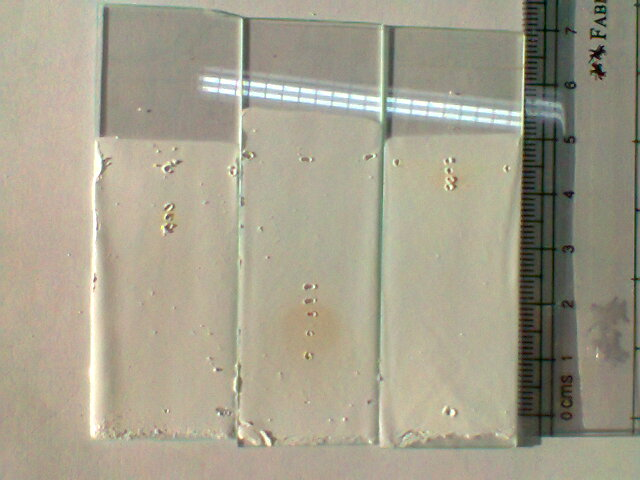
\includegraphics[width=1.2\linewidth]{gfx/e1_1}
		\end{center}
	\caption[TLC plates after Iodine visibility treatment]{\label{1A_slides}}
	\end{figure}


	The $R_f$ value decreases with increase in polarity of the compound being analysed.
\section{Precaution}
	\begin{enumerate}
		\item The slurry shouldn't be very thick
		\item Cover the beakers with a watch glass to ensure there's no loss of volatile substances (minimal that is)
		\item The coating is very fragile, thus the TLC plates must be handled with caution
	\end{enumerate}	
\section{Acknowledgements}
I thank Dr. R Vijaya Anand for his guidance during the experiment. I also acknowledge the contribution of my lab partners, Prashansa and Srijit for performance of the same.